% Bsp. eines Hauptteils

\chapter{Grundlagen}
\label{sec:grundl}

\section{Funktionsprinzip, Vorteile und Herausforderungen des modernen Cloud Computings}

\subsection{Definition und Funktionsweise}

Das National Institute of Standards and Technology (NIST) der Vereinigten
Staaten von Amerika definiert Cloud Computing im Abstract der NIST SP-800-145
folgendermaßen:\\

Cloud computing is a model for enabling ubiquitous, convenient, on-demand network access to a shared
pool of configurable computing resources (e.g., networks, servers, storage, applications, and services) that
can be rapidly provisioned and released with minimal management effort or service provider interaction.
This cloud model is composed of five essential characteristics, three service models, and four deployment
models.\\

Cloud Computing beschreibt ein Modell das es ermöglicht ortsunabhängig, zweckdienlich und
zeitunabhängig auf einen konfigurierbaren Pool an Computerresourcen (Netzwerke, Server,
Datenspeicher, Anwendungen und Services) zuzugreifen die schnell und mit minimalem
Aufwand und minimaler notwendiger Interaktion bereitgestellt und wieder abgebaut
werden können.
Dieses Cloud Modell beschreibt fünf essentielle Charakteristiken, drei Servicemodelle
und vier Bereitstellungsmodelle.\\

Weiter definiert das Dokument die fünf Charakteristiken in den folgenden Punkten:\\

\textbf{On-demand-self-service:} Der Nutzer kann eigenmächtig die benötigten Resourcen
automatisch bereitstellen, es wird keine menschliche Interaktion benötigt.

\textbf{Broad network access:} Auf Leistungen wird über das normale Internet mit standard
Mechanismen die die Nutzung von Thin Clients und Fat Clients (Smartphones, Tablets,
Laptops oder Workstations) fördern zugegriffen.
 
\textbf{Resource Pooling:}: Die Computerresourcen des Anbieters werden in einem gemeinsamen Pool
für mehrere Kunden in einem mandantentauglichen Modell bereitgestellt, physische und
virtuelle Resourcen werden nach dynamisch zugewiesen und entsprechend der Nachfrage
neu verteilt. Es wird eine empfundene Ortsunabhängigkeit hergestellt indem der Nutzer
kein genaues Wissen darüber besitzt wo sich dessen Resources befinden, auf höherem
Level wie beispielsweise dem Staat, der Region oder auch Rechenzentrum kann
der Ort vom Nutzer spezifiziert werden. Die bereitgestellten Resourcen beinhalten
zum Beispiel Datenspeicher, Rechenleistung, Rechenspeicher und Netzwerkbandbreite.

\textbf{Rapid Elasticity:} Rechenkapazitäten werden dehnbar bereitgestellt und abgebaut,
teilweise automatisch, um entsprechend der Nachfrage schnell hoch- und wieder
zurück skalieren zu können, Rechenkapazitäten erscheinen dadurch unbegrenzt und
zu jeder Zeit in jedem Umfang bereitgestellt werden.

\textbf{Measured Service:} Cloud systeme kontrollieren und optimieren Resourcennutzung
automatisch mithilfe eines Messungs-systems dass auf einer abstrakten Ebene den
entsprechenden Service (Datenspeicher, Rechenleistung, Benutzerkonten) überwacht,
kontrolliert und Bericht erstattet um sowohl für Anbieter als auch Kunden Transparenz
herzustellen.\\

Es wird zwischen drei grundlegende Cloud Service Modellen unterschieden: Infrastructure
as a Service (IaaS), Platform as a Service (PaaS) und Software as a Service (SaaS).

\begin{figure}[H]
  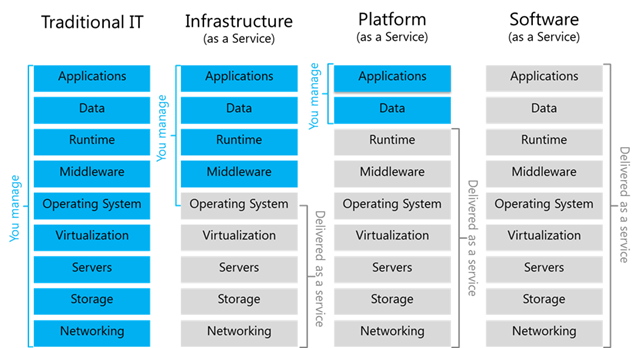
\includegraphics[width=1.0\textwidth]{fig/hauptteil/Service-Models.png}
  \caption{Die grundlegenden Cloud Service Modelle im Überblick}
  \centering
\end{figure}

\textbf{Infrastructure as a Service:} Der Nutzer hat die Fähigkeit Rechenleistung, Datenspeicher
Netzwerke und weitere fundamentale Computerresourcen bereitzustellen und beliebige Software
darauf zu betreiben, dazu können Betriebssysteme und Anwendungen gehören. Die
darunterliegende Infrastruktur wird vom Anbieter betrieben, der Nutzer  kann aber
eingeschränkte Kontrolle über bestimmte Komponenten haben, dazu gehören beispielsweise
Firewalls.

\textbf{Platform as a Service:} Der Nutzer verfügt über die Fähigkeit seine eingkaufte oder
selbst erstellten Anwendungen auf der Cloud Infrastruktur zu betreiben, die notwendige
Umgebung die über Sprachen, Bibliotheken, Tools und Services verfügt wird vom Anbieter
bereitgestellt. Die darunter liegende Infrastruktur mit Netzwerken, Servern,
Betriebssystemen und Speicher wird vom Anbieter betrieben, der Nutzer hat die Kontrolle
über die Anwendung und Konfiguration der Umgebung in der die Anwendung betrieben wird.

\textbf{Software as a Service:} Dem Nutzer wird der Zugriff auf die vom Anbieter in der
Cloud Infrastruktur betriebenen Softwareanwendung gewährt. Auf diese wird mithilfe
eines Thin oder Fat Clients zugegriffen, dabei kümmert sich der Nutzer nicht um den
Betrieb und die Konfiguration der darunterliegenden Cloud Infrastruktur wie
Netzwerke, Server, Betriebssystem, Speicher und die Anwendung selbst mit Ausnahme
eingeschränkter Nutzereinstellungen.

Die von NIST unterschiedenen grundlegenden Service Modellen können noch weiter
differenziert werden.
Ein Beispiel hierfür ist das Modell Function as a Service (FaaS) als Subset von PaaS.
FaaS erlaubt es Programmcode auszuführen ohne sich um die Bereitstellung weiterer 
Infrastruktur kümmern zu müssen wie es der Betrieb eines gewöhnlichen Microservices
verlangt.\\

In Art der Bereitstellung eines Cloud Services werden vier grundlegende Modelle
unterschieden; Public, Private, Hybrid und Community Cloud Modelle.\\

\textbf{Private Cloud:} Die Cloud Infrastruktur wird ausschließlich für die Nutzung durch eine einzige
Organisation mit mehreren Nutzern bereitgestellt. Besitz und Betrieb liegen dabei
entweder bei der selben Organisation, einer Drittpartei oder einer Kombination beider, 
die Infrastruktur kann dabei On- oder Off Premise betrieben werden.

\textbf{Public Cloud:} Die Public Cloud steht für die Nutzung durch die allgemeine Öffentlichkeit bereit.
Die Cloud Infrastruktur befindet sich im Besitz eines Unternehmens, Bildungseinrichtung,
Regierungsorganisation oder einer Kombination aus diesen und wird auch von der selben
Organisation On Premise betrieben. 

\textbf{Community Cloud:} Eine Community Cloud wird von einer Gemeinschaft von Nutzern mit gemeinsamen
Anliegen eingesetzt. Der Besitz und Betrieb liegen dabei bei einem oder mehreren
Mitgliedern dieser Gemeinschaft, einer Drittpartei und kann Off oder On Premise betrieben
werden.

\textbf{Hybrid Cloud:} Die Hybrid Cloud besteht aus einer Kombination der beschriebenen Modelle
(Public, Private und Community). Diese bilden dabei eigene Instanzen die aber durch
standardisierte oder proprietäre Schnittstellen den Transfer von Daten und Anwendungen
zwischen den Instanzen erlauben.

\subsection{Zu erwägende Vor- und Nachteile des Einsatzes von Cloud Computing}

\subsubsection{\textbf{Vorteile und Treiber der Adoption von Cloud Computing}}

\textbf{Wirtschaftliche Vorteile:} Ein Vorteil in der Nutzung von Cloud Computing
kann darin liegen dass ein Großteil der für den Betrieb notwendigen Infrastruktur
nicht mehr vom Unternehmen selbst eingakuft, eingerichtet und betrieben werden
muss (vgl. linke Seite Abb 2.1). Potentiell hohe Kosten die bereits vor der
Inbetriebnahme eines Systems mit einem höheren Risiko aufgewendet werden mussten
stellen in Form von individuell geringeren laufenden Beträgen ein deutlich
reduziertes Risiko da.\\
Sofern der Einsatz von Cloud Computing in einer sinnvollen und korrekten
Weise erfolgt können je nach Fall die Gesamtkosten um einen hohen Anteil reduziert
werden.\\
Die Gesamtkostenersparnisse stehen auch im Zusammenhang mit Skaleneffekten die für
große Cloudanbieter gelten. Der Betrieb eines einzelnen Servers ist im Verhältnis
mit bedeutend höheren Kosten verbunden als das hinzufügen eines äquivalenten
System zu einem Rechenzentrum im Betrieb von AWS oder einem vergleichbaren
Anbieter.

\textbf{Skalierbarkeit:} Besonders für schnell wachsende Unternehmen ist die
Option der schnellen Skalierbarkeit einer der prominentesten Vorteile der Cloud.
Es kann nicht nur auf vorhersagbare Anstiege (zum Beispiel ausgelöst durch
eine Verkaufsaktion) sondern auch auf unvorhersehbare Ereignisse reagiert werden.
Zusätzlich ist es möglich diese Skalierung nicht nur bis zu einem bestimmten Limit,
sondern nahezu unendlich zu betreiben. Wichtig ist auch dass sowohl auf steigende
als auch sinkende Nachfrage reagiert werden kann.

\textbf{Resilienz:} In einem worst case Szenario kann ein ganzes Rechenzentrum
durch unvorhergesehen Ereignisse wie beispielsweise Brände, Naturkatastrophen
oder anderes vollständig zerstört werden. Selbst wenn Backup-Rechenzentren
verfügbar sind ist eine übertragung der Operationen kein trivialer Ablauf und
birgt oft nicht außer Acht zu lassende Risiken. Die Flexibilität der Cloud
erlaubt es die gesamte Infrastruktur mit sehr geringem Aufwand in nicht
betroffene Regionen zu verlagern und die Kontinuität der Geschäftstätigkeiten
mit minimaler Unterbrechung aufrecht zu erhalten.

\textbf{Security:} Security Aspekte können sowohl einen Vor- als auch Nachteil
von Cloud Computings darstellen. Hier sollen zuerst Vorteile dargelegt werden,
potentielle Probleme werden im nächsten Unterkapitel beschrieben.
Die technischen Möglichkeiten und besonders auch die Wahrnung des Themas
Sicherheit in der Cloud unterlagen und unterliegen auch immernoch einem
deutlichen Wandel. Cloud Anbieter investieren
viele Resourcesn in Sicherheit und stellen dem Nutzer zum Beispiel bereits sicher
implementierte Verschlüsselungen zur Verfügung oder bieten einen gewissen
Schutzen vor Denial-of-Service Angriffen durch die natürliche Skalierbarkeit.\\

\subsubsection{\textbf{Nachteile und Risiken}}

\textbf{Netzwerkabhängigeit:} Da der Zugriff auf Cloud Dienste über das
Internet erfolgt entsteht dadurch entsprechend auch eine hohe Abhängigkeit.
Eine stabiele und schnelle Netzwerkanbindung ist vorraussetzung dass effektiv
gearbeitet werden kann, bei lokal gehosteten Systemen ist diese Abhängigkeit
entsprechend geringer.

\textbf{Vendor Lock-in:} Bei der Nutzung eines Cloud Anbieters entsteht die
Gefahr sich zu sehr in Abhängigkeit eines einzelenen Anbieters zu begeben.
Im Fall einer Änderung der Nutzungsbedingungen oder einer Änderung im
Bezahlmodell die den eignen Interessen stark entgegen steht besteht die Gefahr
bereits so abhängig von diesem Anbieter zu sein dass die Kosten eines Wechsels
derart hoch ausfallen dass man gezwungen ist die Bedingugen zu akzeptieren.

\textbf{Security und Privacy:} Sicherheitsrisiken sind einer der meistgenannten
Gründe die gegen Cloud Computing sprechen, besonders im Fall der Nutzung einer
Public Cloud. Die Gefahr dass Daten in die Hände dritter gelangen kann zum
zum Beispiel nicht vollständig ausgeschlossen werden. Da die Verantwortung über
die Sicherheit der Daten dem Cloud Anbieter unterliegt kann es auch zu Problemen
in Hinsicht der Privateheit der Daten kommen, sollte eine Regierungsorganisation
Zugriff auf bestimmte Daten eines Nutzer verlangen könnten diese ohne dessen
Einverständnis gewährt werden.

\textbf{Kosten:} Auch wenn die Nutzung von Cloud Computing mit dem Vorteil
geringerer Kosten beworben ist dies nicht zwingend garantiert. Werden die
vorhandenen Systeme ungünstig verwendet, zum Beispiel bleiben viele gebuchte
Ressourcen ungenutzt und IP-Adressen unverwendet, können hohe Kosten entstehen,
auch in der Phase des Übergangs zu Cloud Computing können höhere Kosten
entstehen als in einem vergleichbaren Zeitraum davor.


\subsection{\textbf{Grundlegende Erklärung von DevOps}}

Die exakte Definition und Abgrenzung des Begriffes DevOps ist ein Thema über
das es keine uniform akzeptierte allein gültige Definition und Abgrenzung gibt.
Im allgemeinen aber bezeichnet DevOps eine stärkere Vereinigung der Entwicklungs-
(Dev) und Betriebs- (Ops) Teams eines Softwareprojekts durch die Anwendung
einer effektiveren Arbeitskultur und -philosophie mit neuen Methoden, Werkzeugen und
Prozessen. Verschiedene Organisationen legen hierbei in ihrer Definition die
Schwerpunkte auf unterschiedliche Aspekte.
Als Beispiel betont Amazon hierbei besonders die schnelle Auslieferung neuer
Produkte ("ability to deliver applications and service at high velocity"),
Microsoft
die Kollaboration zwischen den beteiligten Teams ("DevOps enables formerly
siloed roles - development, IT operations, quality engineering, and security -
to coordinate and collaborate to produce better, more reliable products.").\\
Das DevOps Reasearch and Assessment (DORA) Team
hat über sieben Jahre mit 32.000 Beteiligten die Praktiken und 
Fähigkeiten untersucht die hohe Leistungsfähigkeit bei Entwicklung und
Auslieferung von Sofware fördern. Eine Übersicht über die Erkenntnisse dieser
Studie ist als Diagramm im Anhang ... zu finden.\\
Infrastructure as Code spielt als Werkzeug für die automatisierte Bereitstellung
der benötigten Computerresourcen eine wichtige Rolle im DevOps Prozess.

\subsubsection{\textbf{GitOps als Werkzeug für Continuous Delivery im Rahmen von DevOps}}

GitOps wird von Gitlab als ein betriebliches Rahmenkonzept (operational
Framework) defniert das DevOps Best Practices in der automatiserten
Bereitstellung von Infrastruktur anwendet.
GitOps benötigt dabei drei Hauptkomponenten:\\
Infrastructure as Code, Merge Requests und CI/CD.
Organisationen die mit einer ausgereiften Anwendung der DevOps Kultur arbeiten
können über GitOps hunderte Male pro Tag neuen Code auf den Produktionsservern
installieren. Im praktischen Teil dieser Arbeit wird GitOps verwendet um
da es eine einfache Integration mit Github ermöglicht, Github selbst
wird als Versionskontrollsystem verwendet da es weithin etabliert und breit
unterstützt ist und von der Novatec Consulting GmbH bevorzugt eingesetzt wird.

\subsection{Überblick über die wichtigsten Public Cloud Service Provider}
Da der Kern der Arbeit die Infrastructure as Code Unterstützung der
wichtigsten Cloud Service Provider in deren Public Cloud untersucht soll hier
ein kurzer Überblick über den aktuellen Markt in diesem Bereich gegeben werden.

\begin{figure}[H]
  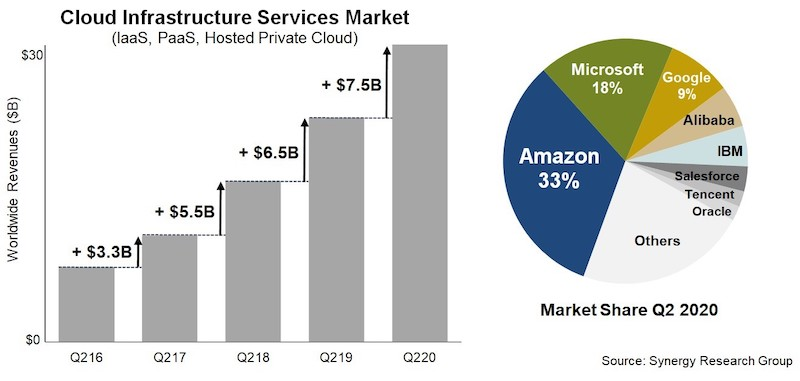
\includegraphics[width=1.0\textwidth]{fig/hauptteil/CIS_Q220.jpg}
  \caption{CSP Market Share Q2 2020 nach Umsatz}
  \centering
\end{figure}

\textbf{1. Amazon: } Amazon besitzt mit 33\% den größten Anteil am Markt.
Die Amazon Elastic Compute Cloud (EC2) ist die älteste der aktuell großen Cloud
Computing Plattformen, der erste Release fand im August 2006 statt.

\textbf{2. Microsoft: } Microsoft stellt den zweitgrößten Anteil am Markt mit
18\%, der erste Release von Microsoft Cloud Computing Service Microsoft Azure
erfolgte im Oktober 2008. Gemeinsam besaßen Amazon und Microsoft 2020 über 50\%
des gesamten Marktes.

\textbf{3. Google: } Google's Google Cloud Platform steht mit 9\% an dritter
Stelle. Google Compute Engine, die IaaS Komponente der Cloud Services von
Google wurde im Juni 2012 veröffentlicht.

\textbf{4. Alibaba Cloud: } Die viertgrößte Cloud Plattform ist die
Alibaba Cloud der Alibaba Group. Alibaba Cloud bietet zusätzlichzu seinem
Elastic Compute Service (ECS) einen dedizierte GPU basierten Service an. 

\textbf{5. IBM Cloud: } Die aktuell fünftgrößte Cloud Computing Plattform ist
die IBM Cloud von IBM. Bis Juni 2013 eine eigene Firma unter dem Namen Softlayer
wurde diese von IBM übernommen und 2017 gemeinsam mit den anderen Cloud Services
der Firma in ein einheitliches Portfolio unter dem Namen IBM Coud aufgenommen.\\

\begin{figure}[H]
  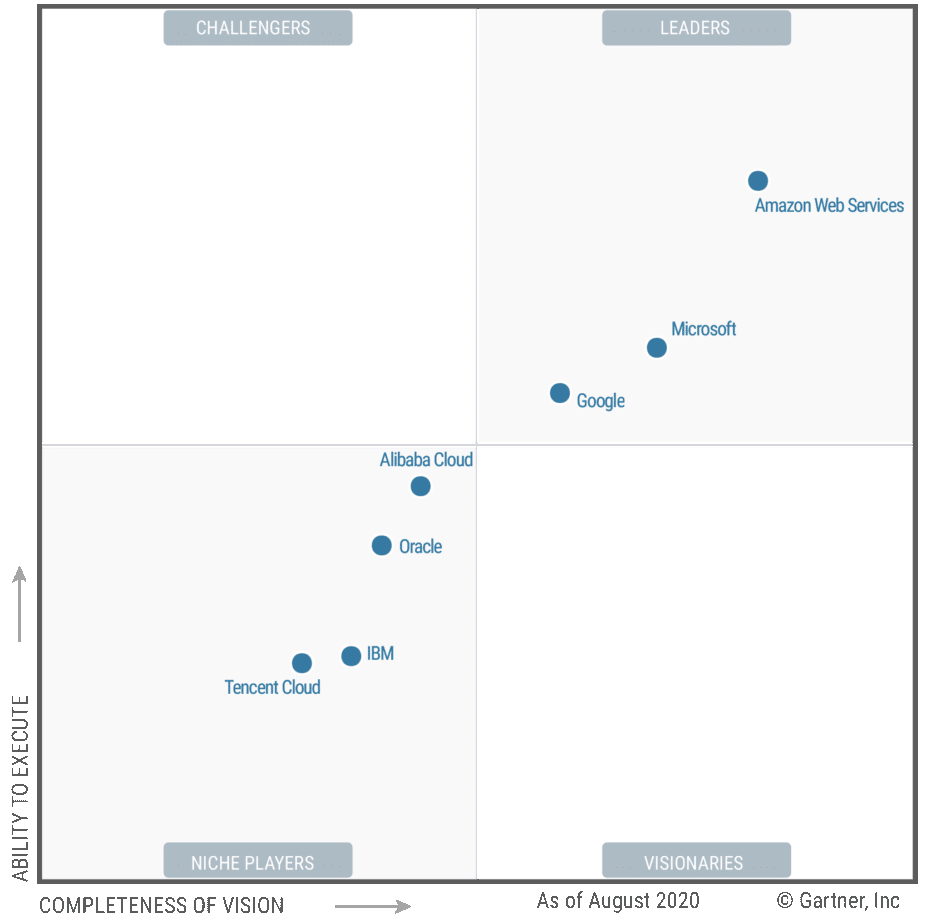
\includegraphics[width=1.0\textwidth]{fig/hauptteil/Gartner-Magic-Quadrant.png}
  \caption{CSP Gartner Magic Quadrant August 2020}
  \centering
\end{figure}

Der Gartner Magic Quadrant für Cloud Service Provider bietet einen groben
Überblick über den Umfang der Angebote (Completeness of Vision) und
die Ausgereiftheit einer Plattform (Ability to Execute). Deutlich erkennbar
ist hier die Vormachtsstellung von Amazon gegenüber Microsoft und Google sowie
der Abstand von Google zum nächst größten Anbieter Alibaba Cloud.
TODO: Irgendwas mit IBM Ability to Execute vs Marktanteil verglichen mit Oracle


\section{Infrastructure as Code}

Infrastructure as Code beschreibt einen Ansatz zur Automatiesierung der
Bereitstellung von Infrastruktur basierend auf Methoden aus der
Softwareentwicklung (vgl Kief Morris Infrastructure as Code S.4).\\
Statt eines manuellen Aufbaus und direkter Konfiguration der einzelnen
Komponenten werden maschinenlesbare Dateien verfasst welche dann von einem
IaC Tool eingelesen und verarbeitet werden. Dabei kommen bevorzugt
deklarative Sprachen zum Einsatz deren höhere Abstraktion mehr Flexibilität
als ein imperativer Ansatz erlaubt.
(vgl. https://docs.microsoft.com/en-us/devops/deliver/what-is-infrastructure-as-code)

\subsection{Technologischer Wandel und das Cloud Age Mindset}

Durch die Technologien der Cloud ist es möglich eine gewünschte
IT-Infrastruktur sehr viel schneller bereitzustellen als
zuvor möglich. Statt des Einkaufs, Anschließens und Einrichtens eines
physischen Servers das, je nach Szenario einen Zeitraum von mindestens
mehreren Stunden oder Tagen bis zu Wochen gedauert hätte können
virtuelle Resourcen in der Cloud in wenigen Minuten bereitgestellt werden.
Der schnellere Ablauf wird durch die Automatisierung von Prozessen wie etwa
der Bereitstellung der Infrastruktur mithilfe von IaC Tools noch verstärkt,
nicht nur bei der initialen 
Mit diesen Veränderungen wird das Management und die Erweiterung der
bestehenden Systeme jedoch nicht unbedingt einfacher (vgl IaC Kief Morris S.3),
die Verwendung der alten IT-Governance Modelle (TODO Fußnotenerklärung) die
sich bisher bewährt haben sind jedoch aufgrund der Veränderungen ungeeignet.
Kief Morris stellt die fundamentalen Unterschiede des Arbeitens mit
Cloud-Technologien mithilfe der folgenden Tabelle dar.

\begin{figure}[H]
  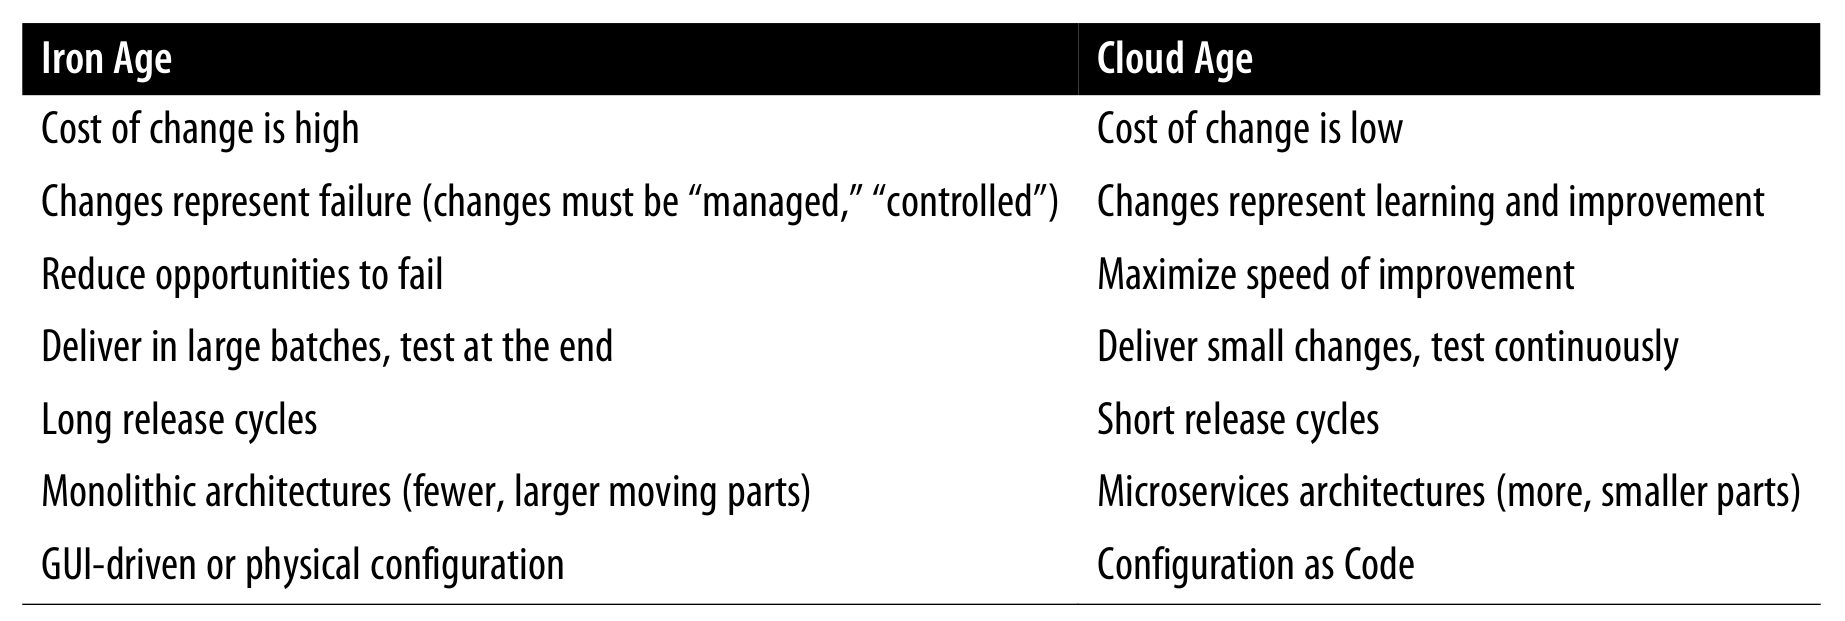
\includegraphics[width=1.0\textwidth]{fig/hauptteil/Tabelle_1-2_IaC.png}
  \caption{Iron Age vs Cloud Age}
  \centering
\end{figure}

Veränderungen in der 'Iron Age' sind aufwändig und teuer und stellen ein
Risiko dar, es wird versucht diese Risikopunkte zu reduzieren daher werden
viele Veränderung gebüdelt getestet und eingeführt wodurch lange
Release-Zyklen entstehen. Die Architekturen die dadurch befördert werden
sind eher monolytisch die Konfiguration erfolgt eher mithilfe von GUI
gesteuerten Programmen oder physischen, zum Beispiel wenn ein neuer Server
in ein Netzwerk eingebunden wird. Veränderungen in der Cloud stellen
fast genau das Gegenteil dar, daher wird erkennbar dass eine auf die
'Iron Age' zugeschnittene Arbeitsweise für die Cloud nicht effektiv ist,
es ist ein neues Cloud Age Mindset das die rechte Spalte der Tabelle
verinnerlicht erforderlich um die Vorteile der Cloud
wirklich effektiv nutzen zu können.

\subsection{Vorteile von IaC und durch IaC gelöste Probleme des
manuellen Provisionings}

\textbf{Kein Configuration Drift durch einheitliche Codebase:}
Configuration drift bezeichnet eine über die Zeit
wachsende Abweichung zweier ursprünglich identischer Systeme. Wird ein
gleiches System, zum Beispiel ein Applikationsserver, in verschiedenen
Umgebungen eingesetzt stellen diese oftmals auch leicht verschiedene
Anforderungen auf die dann mit Optimierungen, etwa in Form spezifischer
Konfigurationsdetails, reagiert werden kann. Wird nun das ursprüngliche
System geupdated werden individuelle, oft undokumentierte Anpassungen
nicht berücksichtigt und ein Update kann unbequeme Konsequenze nach
sich ziehen. Werden alle Veränderungen in einer einheitlichen
Codebase verwaltet und Updates häufig vorgenommen verhindert man
starken Configuration Drift der über Zeit stattfindet

\textbf{Wiederverwendbarkeit durch einheitlichen Code:}
Ein weiterer Vorteil der durch die Verwendung einer einheitlichen
Codebase entsteht ist die Wiederverwendbarkeit und Repoduzierbarkeit
eines Systems. Wenn ein identisches System an einer anderen Stelle
aufgebaut werden soll oder sollte das System aus unvorhergesehen
Gründen in seiner Gesamtheit verloren gehen kann es schnell und mit
verhältnismäßig geringem Aufwand reproduziert werden.
Ein dazu passender Ausdruck in Bezug auf Server ist 'Cattle not Pets'.
Statt sich individuell und mit großem Aufwand um einzelne Server zu
kümmern wie man es etwa mit dem eigenen Haustier tut sollten Server
wie leicht ersetzbares Vieh behandelt werden.

\textbf{Schnelleres Provisioning durch Cloud:} Ein bereits häufig
angesprochener Vorteil ist die schnelle Bereitstellung, auf tiefere
Erklärung kann daher hier verzichtet werden.

\textbf{Schnellerer Profit:} Schnellere Bereitstellung der Hardware
und schnellere Auslieferung von Software die durch DevOps Methoden
begünstigt werden erzeugen entsprechend auch schneller einen Mehrwert.

\textbf{Einheitliches Tooling in Dev, Ops und weiteren Beteiligten Teams:}
Verwendung von IaC
fördert die einheitlicheres Tooling in allen Bereichen die mit einem
Softwareprodukt in Zusammenhang stehen. Cloud Technologien fördern und
ermöglichen diese Vereinheitlichung, manuelles Provisioning ohne ein
Cloud Modell erschwert dies oder macht es sogar unmöglich.

\textbf{Stärkere Automatisierung im Arbeitsablauf:} Automatisierung
bedeutet immer einen gewissen upfront Overhead, jedoch kann auf
längere Sicht deutlich von automatisierten Abläufen profitiert weren.
Ein Beispiel hierfür sind automatisierte und in eine CI/CD Pipeline
integrierte Tests.

\textbf{Höhere Zuverlässigkeit und Sicherheit durch schnelle Updates:}
Von eine Struktur die schnelle und häufige Veränderungen fördert
kann auch die Sicherheit und Zuverlässigkeit eines Systems profitieren.
Auf Sicherheitsrisiken kann in kurzer Zeit und ohne viel Aufwand
reagiert werden, eine unsichere Funktion kann etwa schnell durch
eine sichere Variante ausgetauscht werden, mögliche damit verbundene
Probleme können dann in automatisierten Tests erkannt werden wodurch
das System zuverlässig bleibt.

\textbf{Schnellere Fehlersuche und -behebung:}

Fehler die dennoch auftreten können dann durch den Einsatz kleinerer
Komponenten schneller isoliert, gefunden und behoben werden.
Monolithische Systeme erschweren dies durch dadurch dass weniger klar
isolierte Komponenten vorhanden sind die häufig mehr Abhängigkeiten
aufweisen und daher schwerer als einzelne Einheit getestet werden können.

\subsection{Herausforderungen und Argumente gegen den Einsatz von IaC}

Kief Morris bennent drei Argumente die gegen die Einführung von IaC
genannt werden, diese sollen hier Im Kontext der gennanten Vorteile betrachtet
werden.

\textbf{Veränderugen werden nicht oft genug durchgeführt um
Automatisierung zu rechtfertigen.}

Die Idee dass ein System einmal erstellt und dann "fertig" ist und
Automatisierung der Veränderungen daher überflüssig ist 
entspricht sehr selten der tatsächlichen Realität.
IT-Systeme und damit auch IT-Infrastruktur wird während ihrem gesamten
Lebenszyklus mehr oder weniger kontinuierlich verändert und erweitert.\\
Sicherheislücken in alten Versionen von Softwarepackages oder
Betriebssystemen sind keine Seltenheit und müssen gepatcht werden um
einen sicheren und Zuverlässig Betrieb zu gewährleisten, neue Features
in bestehender Software kann neue Infrastruktur, zum Beispiel in Form eines
neuen Datnbankservers, notwendig machen oder eine veränderte Konfiguration
ist nötig um die Performance zu steigern. Gerade bei Sicherheitslücken
ist es wichtig Anpassungen nicht erst nach längerer Zeit sondern so
schnell wie möglich durchzuführen um Sicherheit und Stabilität nicht
zu gefährden. Ein weiteres Szenario das die Stabilität eines Systems
gefährden kann ist ein schneller Zuwachs an Last die das System erfährt,
daher sollte es möglich schnell und unkompliziert das System zu verändern
indem mehr Resourcen zur Verfügung gestellt werden.

"A fundamental truth of the Cloud Age is: Stablity comes from making changes."
(IaC Buch S. 5)

Eine fundamentale Wahrheit des Cloud Zeitalters ist: Stabilität ensteht durch
Veränderung.

\textbf{Infrastruktur soll zuerst aufgebaut, danach automatisiert werden.}

Die Umsetzung von Infrastructure as Code stellt eine durchaus große
Herausforderung, das Erlernen eine "steep Curve" (IaC Buch S.6) dar, deren
Nutzen nicht unbedingt direkt ersichtlich ist. Dadurch kommt es zu
Situationen in denen es attraktiv erscheint Infrastruktur zuerst aufzubauen
sich erst später um die Automatisierung zu kümmern. Mit diesem
Ansatz werden viele der Vorteile von IaC jedoch verwirkt und die Schwierigkeit
der Umsetzung von IaC fällt deutlich größer aus, verglichen mit einem
Projekt das von Beginn auf IaC ausgelegt ist da 
"Automatisierung Teil des Designs und der Implementierungeines Systems ist"
(IaC Buch S.6).\\
Automatisierung mit IaC vereinfacht auch die Implementierung autoamtisierter
Tests eines Systems was es wiederum erlaubt Fehler schneller zu beheben.
Ist dies bereits von Beginn an Teil des Arbeitsprozesses verbessert dies
die Qualität der Infrastruktur.\\

TODO: Wenn erfolgreich werden neue Features gefordert, ohne Automatisierung
gerät Management der wachsenden Infrastruktur schnell außer Kontrolle
Deliver steady stream of value , build system incrementally

\textbf{Es muss zwischen schneller Umsetzung und hoher Qualität
gewählt werden.}

Die Idee dass der Fokus auf hohe Geschwindigkeit und hohe Qualität
sich gegenseitig behindert oder ausschließt mag logisch erscheinen,
in der Praxis ist dies jedoch nicht der Fall.
Die "Accelerate State of DevOps Report" Studie kam zu dem Schluss
das Organisationen dazu tendieren entweder gut oder schlecht in beiden
Kriterien abzuschneiden, wird eines vernachlässigt führt es am Ende
in der Regel zu einem "fragile Mess" wie die untenstehende Tabelle
erläutert.

\begin{figure}[H]
  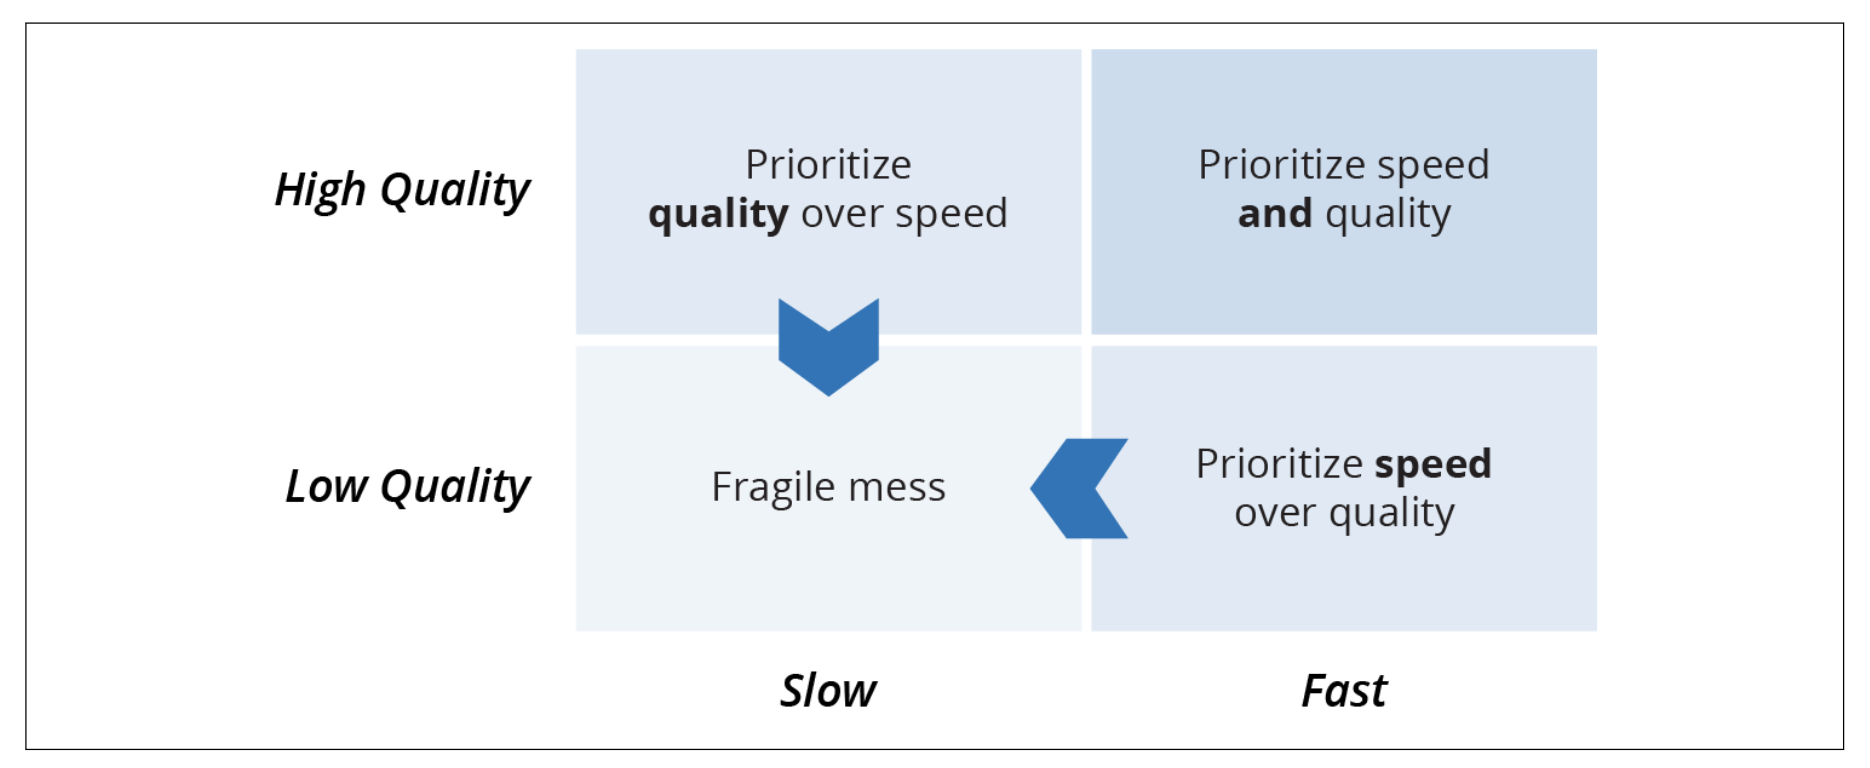
\includegraphics[width=1.0\textwidth]{fig/hauptteil/Speed_vs_Quality.png}
  \caption{Iron Age vs Cloud Age IaC Busch S.6}
  \centering
\end{figure}

Wird Geschwindgkeit über Qualität gestellt (Quadrant links oben) entstehen
mit der Zeit chaotische und instabiele Systeme an denen Veränderungen mit
der Zeit nur noch erschwert und deshalb langsam durchgeführt werden können.\\
Wird Geschwindigkeit zu niedrig priorisiert führt es allerdings auch dazu
dass letzten Endes durch Druck von Deadlines und schnellen workarounds
technische Schulden aufgebaut werden die ebenfalls zu einem qualitativ
schlechten System führen da notwendige Veränderungen nicht schnell genug
eingearbeitet werden können.

Aufgrund dieser Probleme ist es wichtig Geschwindgkeit und Qualität
gleichermaßen zu priorisieren, moderne Entwicklungsansätze DevOps
haben das Ziel dies zu erreichen, der Erfolg wird von der
Accelerate Studie belegt.

\subsection{Die drei Kernverfahren von IaC}

Kief Morris identifiziert drei Kernverfahren ("Core Practices")
zur Implementierung von Infrastructure as Code:

\begin{itemize} 
  \item \textbf{Define everything as Code:} Alle Teile eines System
  in Form von Code zu definieren bringt mehrere Vorteile mit sich.\\
  Code kann mehrfach ausgeführt werden, daher ist eine als Code
  definieres System Wiederverwendebar. Es können unkompliziert mehrere
  identische Instanzen erstellt werden, das Gilt auch für den Fall
  wenn Fehler auftreten und ein Neuaufbau erforderlich ist.
  Das Verhalten des Systems ist vohersehbar, fortlaufendes automatisches
  Testen ist möglich und damit auch zuverlässiger.\\
  Definition in Code macht auch den Aufbau eines Systems transparenter,
  da dieser immer dem tatsächlichen Zustand des Systems entspricht und
  damit auch dokumentiert.
  
  \item \textbf{Continuously Test and Deliver All Work in Progress:} 
  Fortlaufendes, automatisiertes Testen und Integrieren aller Komponenten
  die sich in Entwicklung befinden dient dem Ziel die Qualität eines
  Systems nicht nur "einzutesten" sondern von Beginn and und kontnuierlich
  einzubauen
  (The idea is to build quality in rather than trying to test quality in.
  (vgl IaC Buch S.10)). Nach der Accelerate Studie fördert es die Qualität
  der Arbeit eines Teams wenn jedes Mitglied mindestens einmal am Tag den
  eigenen Fortschritt integriert.

  \item \textbf{Build Small, Simple Pieces That You Can Change Independently:} 
  Systeme die aus mehreren kleineren voneinander unabhängigen Komponenten
  bestehen sind generell stabieler als große Monolithen. Eine Änderung die
  einen Fehler verursacht betrifft nur diese Komponente in der die Änderung
  stattfindet, diese kann dann leichter isoliert und das Problem behoben
  werden, kleine Komponenten sind in der Regel auch weniger Komplex und
  dadurch leichter zu verstehen. Ein einzelner Fehler nach einem Update
  hat auch den Vorteil dass nur diese Komponente und nicht das gesamte
  restliche System auf eine ältere Version zurückgesetzt werden muss um
  den Betrieb wieder herzustellen.

\end{itemize}

\subsection{Die Rolle von Terraform im IaC Anwendungsprozess}

Während der Anwendung von Infrastructure as Code kann primär zwischen zwei
wichtigen Phasen unterschieden werden, einer initialen Einrichtungsphase
und der darauf folgenden Wartungs- und Betriebsphase.\\
In der Einrichtung wird die Infrastruktur bereitgestellt und konfiguriert,
genauso wird auch Software intalliert und eingerichtet.\\
Nachdem das System dann in Betrieb genommen wurde können Anpassung notwendig
werden, Server werden hinzugefügt und abgebaut, Software wird aktualisiert
und neu konfiguriert.

\subsubsection{Überblick über die wichtigsten Infrastructure as Code Tools}

Infrastructre as Code beinhaltet verschiedene konkrete Anwendungsfälle und
entsprechend existieren auch Tools die zum Teil ein breiteres Spektrum
von IaC abdecken, zum Teil aber auch eher spezialisiert sind; Terraform
ist dabei ein Beispiel für ein spezialisierteres Tool. Die untenstehende
Abbildung soll einen Überblick über die aktuell relevantesten Tools
verschaffen, die Einordnungen sind dabei aber nicht unbedingt als absolut
anzusehen. Es ist zum Beispiel möglich innerhalb eines Terraform-Deployments
auch Software zu installieren und zu konfigurieren, allerdings wird die
tatsächliche Installation dann eher per von Terraform aufgerufenen Skripten
vorgenommen statt von Terraform selbst verwaltet zu werden, daher ist
Terraform hier ausschließlich als Infrastruktur-Management Tool eingeordnet.

\begin{figure}[H]
  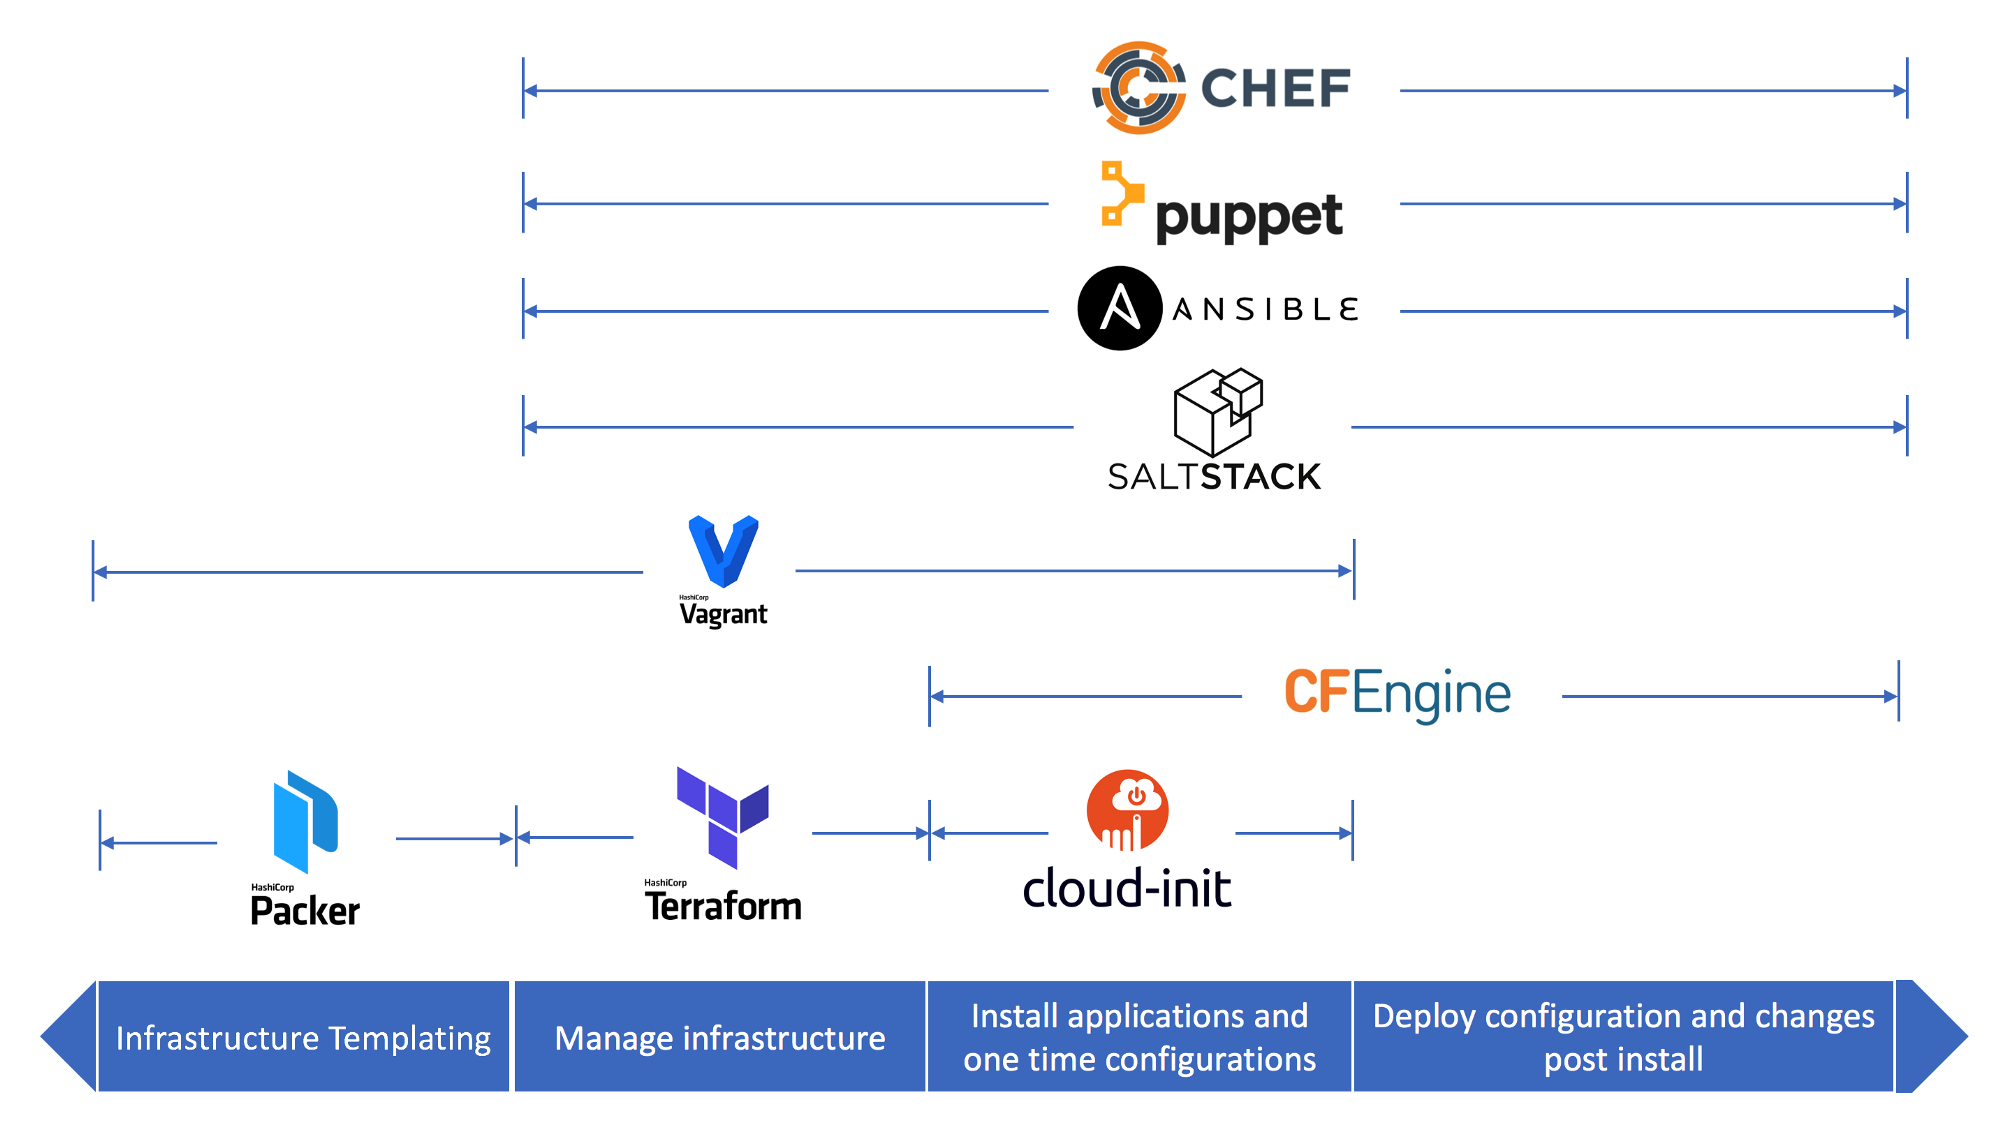
\includegraphics[width=1.0\textwidth]{fig/hauptteil/IaC_Tools.png}
  \caption{Überblick IaC Tools https://medium.com/cloudnativeinfra/when-to-use-which-infrastructure-as-code-tool-665af289fbde}
  \centering
\end{figure}

\subsubsection{Vorteile und Limiterungen von Terraform}

Da sich diese Arbeit primär mit dem Provisioning von grundlegender Cloud
Computing Infrastruktur in Form von VM's, Netzwerken, Datenspeicher und
anderen grundlegenden Komponenten beschäftigen soll bietet sich der Einsatz
eines darauf spezialisierten Tools an.\\
Hier gibt es zusätzlich zu Terraform eine weitere prominente Alternative:
Pulumi.

Pulumi bietet im Vergleich zu Terraform mehrere Vorteile, es gibt allerdings
auch diverse Nachteile die, gegen den Einsatz von
Pulumi sprechen. Die folgenden Vorteile bietet Pulumi gegenüber Terraform:

\begin{itemize}
  \item \textbf{Sprache:} Im Gegensatz zu Terraforms Domänen-spezifischer
  HashiCorp Configuration Language (HCL) setzt Pulumi auf den Einsatz
  bekannter General-Purpose Programmiersprachen, Python, TypeScript,
  JavaScript, Go, C\# und F\#, werden aktuell unterstützt.\\
  Durch den Einsatz dieser Sprachen können Schleifen, Funktionen und
  weitere bekannte Konstrukte verwendet werden, Terraform bietet diese
  Möglichkeiten nicht, ähnliche Effekte werden nur mit Workarounds erreicht.

  \item \textbf{Testing:} Um Terraform-code testen zu können werden
  Third-party Tools benötigt, Terraform selbst bietet kein Test-Framework.
  Durch den Einsatz bekannter General-Purpose Programmiersprachen in Pulumi
  ist es auch möglich die dort zum Einsatz kommenden Frameworks zu verwenden,
  Integrationstest sind allerdings nur in Go unterstützt
  (https://phoenixnap.com/blog/pulumi-vs-terraform).
  
  \item \textbf{Pulumi mit Terraform:} Pulumi kann kann sowohl lokale als auch
  remote Terraform State Files lesen und verarbeiten. Dies erlaubt es Pulumi
  und Terraform nebeneinander einzusetzen um verschiedene Teile der
  Infrastruktur mit dem jeweils anderen Tool zu managen, soll zum Beispiel 
  einer Umstellung von Terraform auf Pulumi erfolgen ist dies möglich
  ohne das gesamte System auf einmal auser Betrieb nehmen zu müssen.

\end{itemize}

Terraform wiederum bietet die folgenden Vorteile:

\begin{itemize}
  \item \textbf{Modularität:} Terraform Module erlauben es ein System in
  mehrere klar definierte Komponenten zu strukturieren, dadurch wird die
  Wiederverwendbarkeit dieser Komponenten ermöglicht und gefördert.
  Die daraus resultierenden Vorteile wurden bereits in den vorangegangenen
  Kapiteln dargelegt, daher soll hier nicht weiter darauf eingegangen werden.
  Pulumi strukturiert Infrastruktur Code entweder in einem großen
  monolithischen Projekt oder vielen kleinen Mikroprojekten, beide
  Optionen sind weniger flexibel als die Lösung die Terraform bietet.

  \item \textbf{State Debugging:} Es ist beinahe unvermeidbar
  dass es während der Arbeit an einem Infrastrukturprojekt über einen
  längeren Zeitraum irgendwann einmal zu einem Fehler im State kommt.
  Sowohl Terraform als auch Pulumi bieten hier CLI Befehle die bei der
  Fehlersuche und -behebung unterstützen, Terraform bietet hier jedoch
  aktuell noch mehr Optione mit denen Resourcen aus dem aktuellen State
  gelöscht oder hinzugefügt werden können, dadurch wird weniger händische,
  und potentiell fehleranfälligere Arbeit direkt im State File notwendig.

  \item \textbf{Weitere Verbreitung und größere Popularität:} Terraform wurde
  2014, Pulumi 2017 veröffentlicht, entsprechend ist Terraform deutlich weiter
  verbreitet und verfügt über all die Vorteile die eine größere Community mit
  sich bringt. Dazu gehören mehr Lernresourcen, mehr Codebeispiele, größere
  Bekanntheit und mehr Jobs für die Arbeit mit Terraform.

  \item \textbf{Dokumentation:} Einen weiteren Voteil von Terraform stellt
  dessen umfangreiche und ausgereifte Dokumentation sowie auch die
  Dokumentation der einzelnen Provider dar. Der genaue Aufbau der einzelnen
  Resourcen wie etwa einer VM auf Google Cloud Platform
  (google\_compute\_instance) ist mit einem Beispiel und der zugehörigen
  Argument Reference versehen aus der direkt ersichtlich wird welche
  Argumente notwendig (required), was der Zweck jedes einzelnen Arguments ist
  und wo anstelle eines einfachen Wertes ein Block erwartet wird.

\end{itemize}

-Terraform unterm Strich aktuell interessanter für große Projekte/Unternehmen
=> daher Wahl für diese Arbeit

- Ein wirklich fundierter Vergleich zwischen Terraform und Pulumi benötigt
deutlich mehr Zeit und Anspruch als im Rahmen dieser Arbeit möglich, für
die in diesem Fall und zu diesem Zeitpunkt zu treffende Entscheidung soll
der grobe Vergleich hier ausreichen. Ein umfangreicherer Vergleich zwischen
Terraform und Pulumi könnte in zwei Jahren ein anderes Ergebnis liefern
als heute, beide Technologien und insbesondere Pulumi sind noch relativ neu
und nicht vollständig ausgereift.

\subsubsection{Weitere zu beachtendende Aspekte}

Ein Aspekt über Terraform der häufig falsch interpretiert und verbreitet wird
ist dass Terrafom als Cloud agnostisch beschrieben ist. Dies ist NICHT der
Fall. Die einzelnen Terraform Provider welche jeweils die Abstraktion der
Cloud Service Provider tatsächlich vornehmen sind nicht austauschbar das heißt
der Terraform Code muss für jeden Cloud Service Provider individuell
geschrieben werden, Terraform Code ist daher nicht Cloud agnostisch.\\

(- Secrets Management? Terraform Enterprise?)

\subsection{Terraform Funktionsprinzip}

Terraform ist ein Infrastructure as Code Tool das es ermöglicht Infrastruktur
sicher und effizient aufzubauen, zu verändern und zu versionieren.\\
Terraform verwendet eine High-level DSL die es erlaubt die Infrastruktur in
deklarativer und menschenlesbaren Konfigurationsdateien zu beschreiben die
versioniert, geteilt und wiederverwendet werden können.\\
Bevor Veränderungen vorgenommen werden erzeugt Terraform einen Execution
Plan der beschreibt welche Veränderungen durchgeführt werden sollen und
überprüft werden kann bevor er ausgeführt wird.\\
Ein Resourcengraph der Abhängigkeiten erfasst erlaubt es voneinander
unabhängige Resourcen parallel und dadurch effizient zu erzeugen und gibt
einen besseren Einblick in den Aufbau des beschriebenen Systems.\\
Automatisierte Änderungen erlauben es komplexe Veränderungen an der
Infrastruktur mit minimaler menschlicher Interkation durchzuführen.
Terraform beachtet bestehende Abhängigkeiten und nimmt Veränderungen
durch Execution Plans schrittweise vor bis der definierte Zustand erreicht
ist. (Alles obere vgl https://www.terraform.io/intro/index.html)

Die folgende Abbildung stellt das Funktionsprinzip von Terraform mit den
wichtigsten beteiligten Komponenten dar.

\begin{figure}[H]
  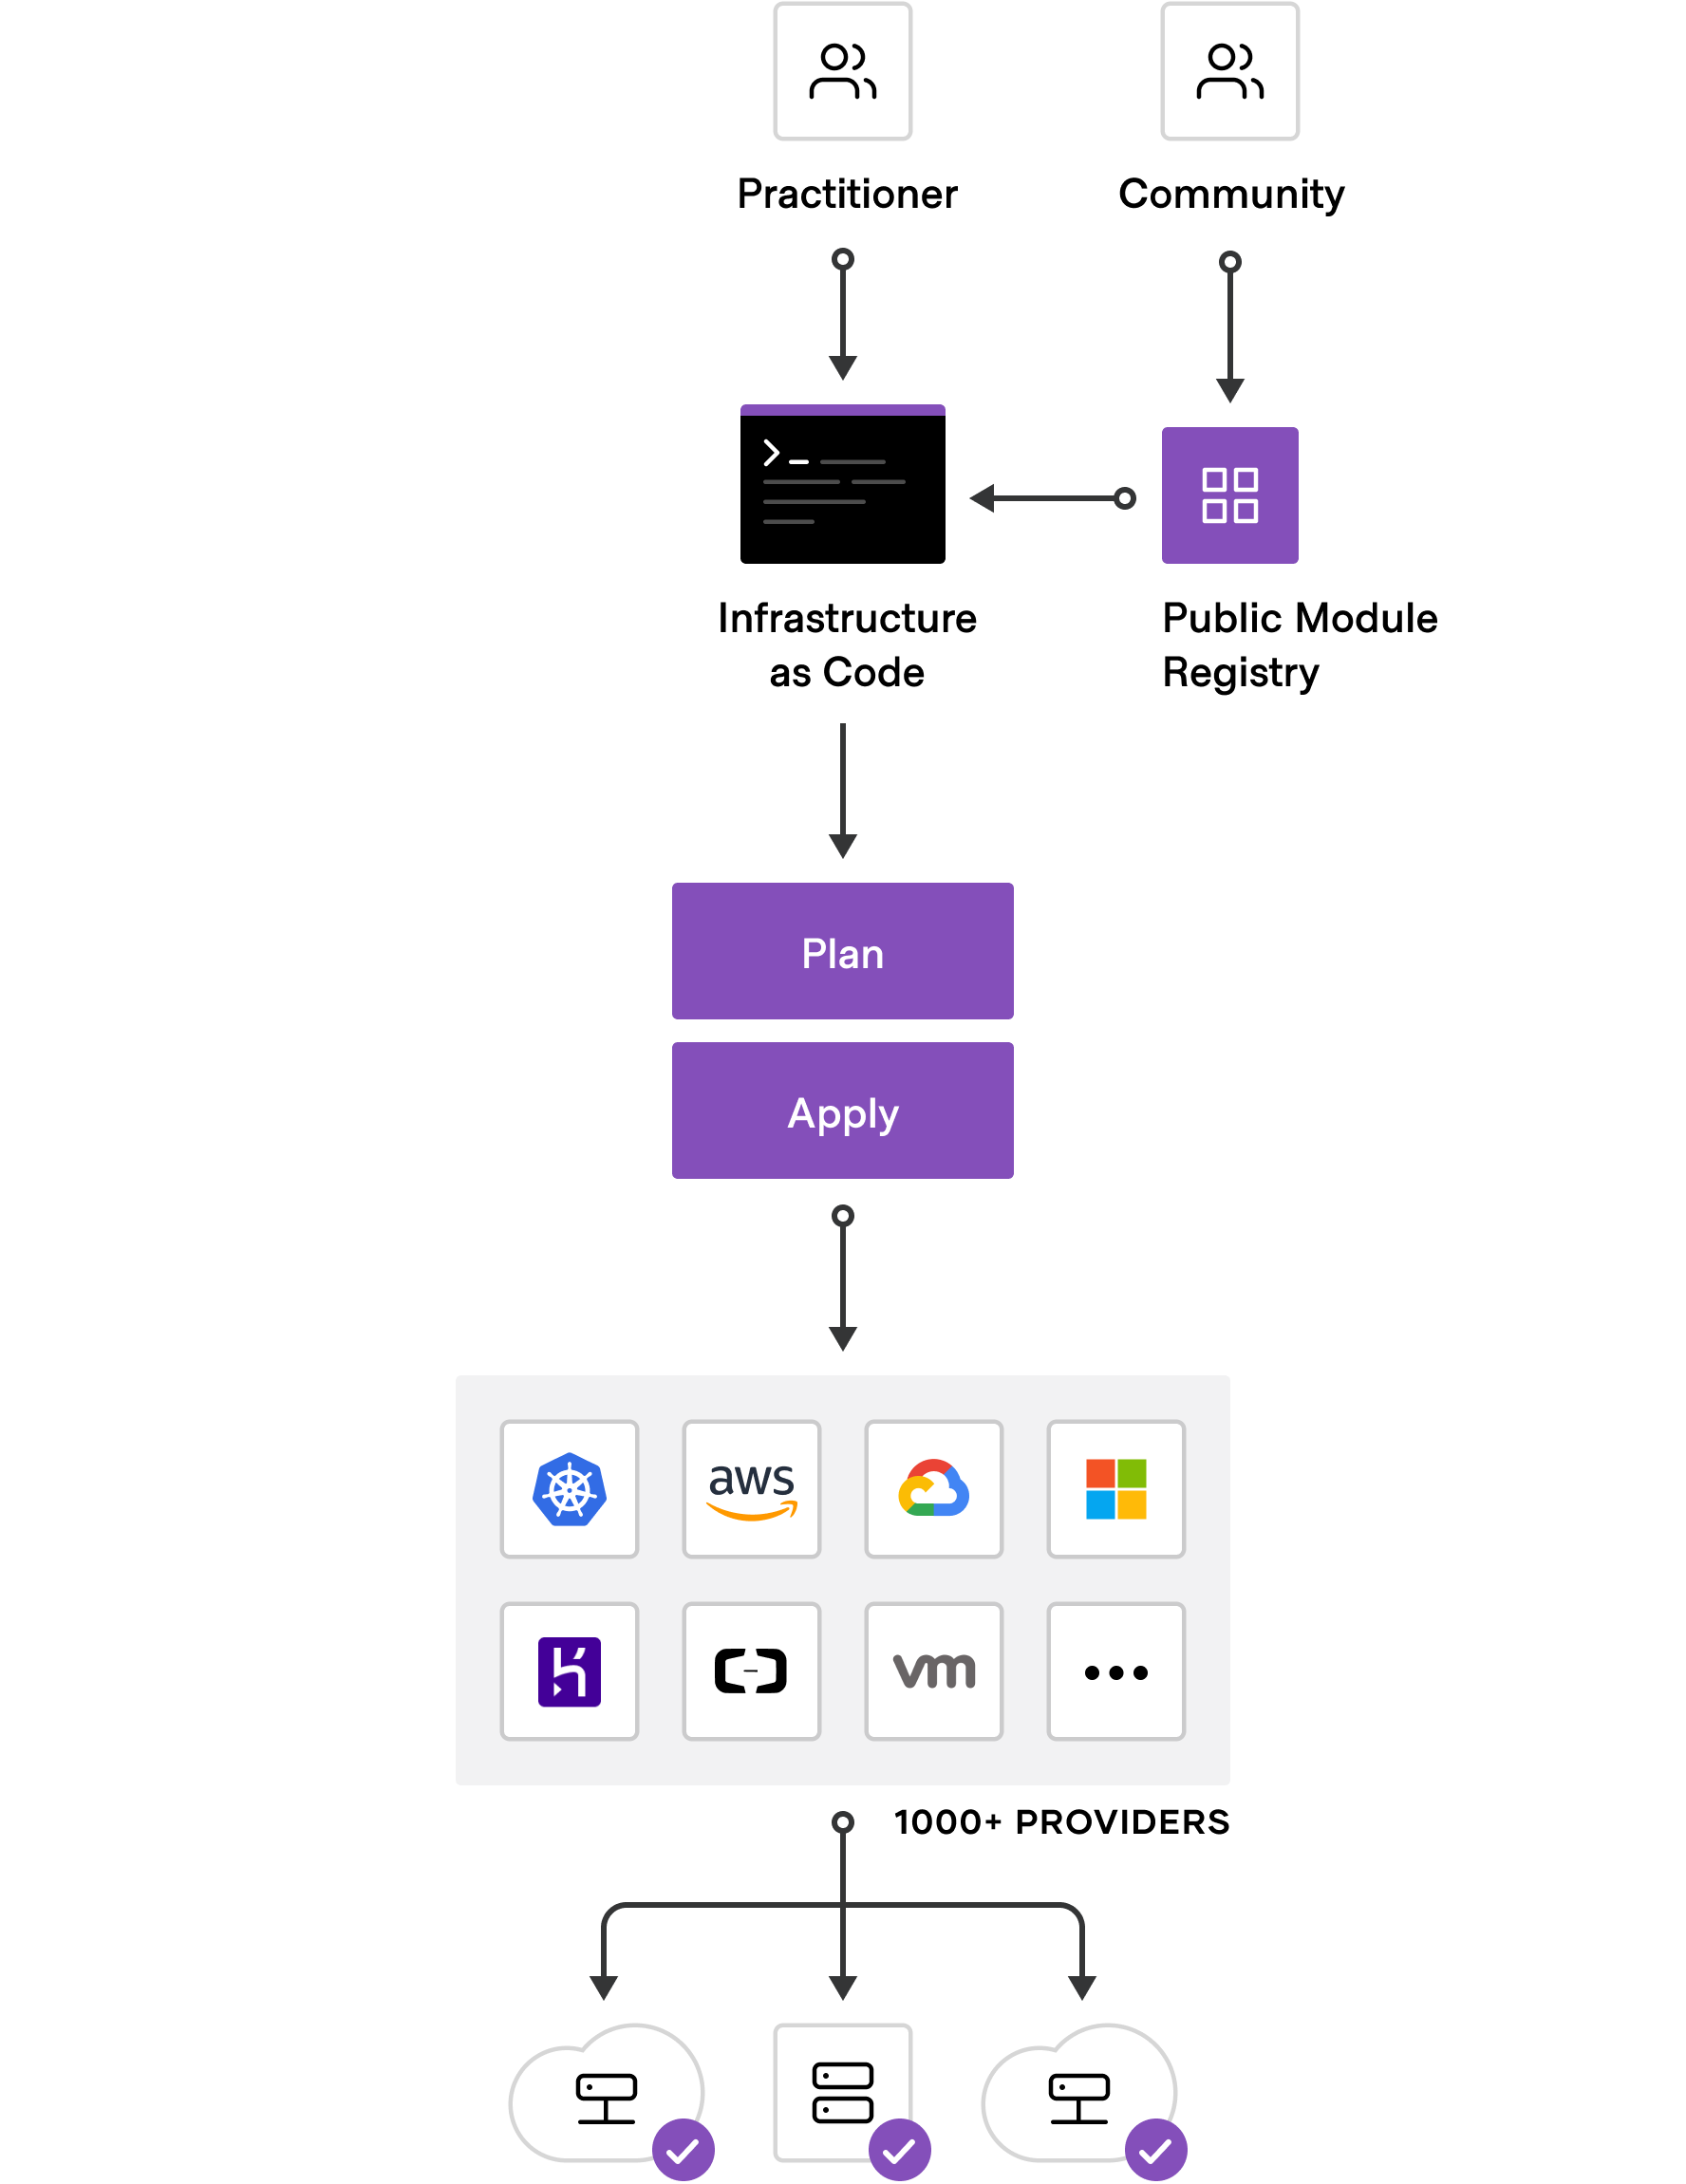
\includegraphics[keepaspectratio, height=15cm]{fig/hauptteil/Terraform.png}
  \caption{Terraform Funktionsprinzip}
  \centering
\end{figure}

Der Terraform Anwender schreibt den Infrastruktur Code in HCL. Dabei kann
er auf vorhandene Module aus der Public Module Registry zurückgreifen um
typische Strukturen wie Netzwerke aufzubauen. Die Terraform Core-Software
nutzt dann Plugins, die Terraform Provider, um die jeweiligen Cloud Plattform
API's anzusprechen die dann die Infrastrktur aufbauen. Die aktuell
existierenden Resourcen sind dabei in der terraform.tfstate Datei
festgehalten, gemeinsam mit dem aktuellen State und dem Infrastruktur Code
ermittelt Terraform welche Änderungen vorgenommen werden müssen um den
im Code beschriebenen Zustand zu erreichen.

\subsubsection{Hashicorp Configuration Language}

Die von Terraform verwendete Konfigurationssprache wurde mit dem Ziel
entwickelt einen Kompromiss zwischen Maschinenfreundlichkeit und
Menschenlesbarkeit zu erzielen. Existierende Serialisierungsformate,
Konfigurationssprachen und Programmiersprachen konnten die Ziele
der Terraform-Entwickler nicht erfüllen daher kommt nun bei Terraform
eine DSL in Form der Hashicorp Configuration Language zum Einsatz.

HCL besteht aus drei grundlegenden Elementen: Blöcken (Blocks), Argumenten
(Arguments) und Ausdrücken (Expressions).

TODO Codebeispiel

\textbf{Blöcke} stellen für gewöhnlich ein Objekt, im Fall von
Infrastrkturcode meistens eine Computing Resource, dar.
Blöcke besitzen einen Typ und Null bis mehrere label. Blöcke beinhalten
Argumente und weitere verschachtelte Blöcke.\\
\textbf{Argumente} sind das was in den meisten Programmiersprachen die
Variablen darstellen: Ein Wert der einem Namen zugewiesen wird.\\
\textbf{Ausdrücke} sind ähnlich wie in anderen Sprachen ein aus anderen
Ausdrücken und Argumenten berechneter Wert, ein Argument ist in diesem Sinne
die simpelste For eines Ausdrucks.

\subsubsection{Input und Output Variablen}

Input Variables sind nützlich um Parameter außerhalb des eigentlichen
Terraform Codes anzupassen. Die ID des Projektes stellt einen solchen
Parameter dar, befindet sich diese außerhalb des Codes muss nur die Datei
welche die Inputvariablen enthält angepasst werden, alles andere kann ohne
Veränderungen wiederverwendet werden.

TODO Codebeispiel

Inputvariablen sind einfache Key-Value Paare die einen Standardwert und
eine optionale Beschreibung besitzen.

Outputvariablen werden in der Regel verwendet um auf spezifische Parameter
einfachen und schnellen Zugriff zu ermöglichen.

TODO Codebeispiel

Werte wie die IP einer
Virtuellen Maschine auf einer Public Cloud Plattform sind vor der
Bereitstellung dieser nicht bekannt, werden aber häufig benötigt weshalb es
nützlich ist eine Output Variable für diese zu deklarieren.

\subsubsection{Terraform Module}

Module sind Container für mehrere Resourcen die gemeinsam verwendet werden.
Jedes Terraform Projekt besitzt ein Root Module das weitere Module verwenden
kann. Die Terraform Registry stellt eine Vielzahl an veröffentlichten
Modulen zur öfentlichen Verwendung bereit.

\subsubsection{Terraform Provider}

Terraform benötigt Plugins, die Provider, um mit Cloud Providern,
SaaS Providern und anderen API's interagieren zu können. (vgl https://www.terraform.io/docs/language/providers/index.html)
Provider ermöglichen es Terraform für gewöhnlich einen bestimmten Provider zu
konfigurieren, es gibt zum Beispiel einen Provider für Google Cloud
Platform, es gibt aber auch Provider die eine lokales Utility Tool für die
Nutzung durch Terraform konfigurieren. Öffentliche Provider werden primär
auf der Terraform Registry bereitgestellt und dokumentiert.

\subsubsection{Terraform Workflow}

Der grundlegende Terraform Workflow besteht aus vier Schritten:

TODO Code terraform init

Das init Kommando installiert und konfiguriert die notwendigen Provider
und Module und konfiguriert ein Backend (Fußnote Backend) falls angegeben.

TODO Code terraform plan

Mit terraform plan wird ein Execution Plan erstellt. Dazu gehört den die
aktuell existierenden Resourcen zu erfassen, Veränderungen zwischen
diesem Zustand und dem im Code konfigurierten Zustand zu erfassen und
auf Grundlage dessen einen Plan zu erstellen welche Änderungen vorgenommen
werden können um den Soll-Zustand zu erreichen.

Todo Code terraform apply

Durch terraform apply wird ein solcher Execution Plan ausgeführt und die darin
enthaltenen Änderungen an der Infrastruktur vorgenommen.

Todo Code terraform destroy

Um den umkomplizierten Abbau eines mit Terraform definierten und aufgebauten
Systems bewerkstelligen zu können wird das terraform destroy Kommando
verwendet. Dies ist besonders nützlich um nicht mehr benötigte Testsysteme
und andere temporäre Infrastrukturen zu entfernen.

\chapter{Aufbau und Untersuchung}
\label{sec:real}
Beschreibung der HW- und SW-Realisierung

\section{High-level Aufbau der Infrastruktur des Versuchsobjekts}
\label{sec:real-unter}
Beispiel Text

\section{Zu analysiernde Aspekte und Eigenschaften}

\section{Konkreter Aufbau in Microsoft Azure}

\section{Analyse Azure}

\section{Konkreter Aufbau in Amazon AWS}

\section{Analyse AWS}

\section{Konkreter Aufbau in Google Cloud Platform}

\section{Analyse GCP}

\section{Literaturverweise}
\label{sec:real-literatur}

Verweise im Text: \cite{doc:stz} und \cite{doc:gun}.

\chapter{Ergebnisse}
\label{sec:ergeb}


\section{Resultate und Vergleichsmatrix}

\enquote{Neuigkeiten} Messergebnisse
